\chapter{Introduction}
\label{cha:intro}

% TODO: The first chapter contains a general introduction to the work. The goals are defined and the modus operandi is explained.

The mobile industry is without a doubt one of the most vibrant industries at the moment. Not only because mobile device sales are growing rapidly but also because of the highly competitive nature of this market. This has led to fragmentation. 

This chapter will sketch the landscape of mobile devices, explain the problem of fragmentation and a number of suggested solutions to cope with this problem.

\section{The mobile device landscape}

In the last couple of years, smartphone sales have gone up quickly. Smartphones are becoming ubiquitous and in some regions, like the United States, smartphone penetration has already reached more than 50\% \cite{Nielsen:2012}. According to quarterly studies by Gartner, smartphone penetration remained stable before the iPhone 3G and Android came along (see \fref{fig:smartphone_sales}).

\begin{figure}[h!]
    \begin{center}
        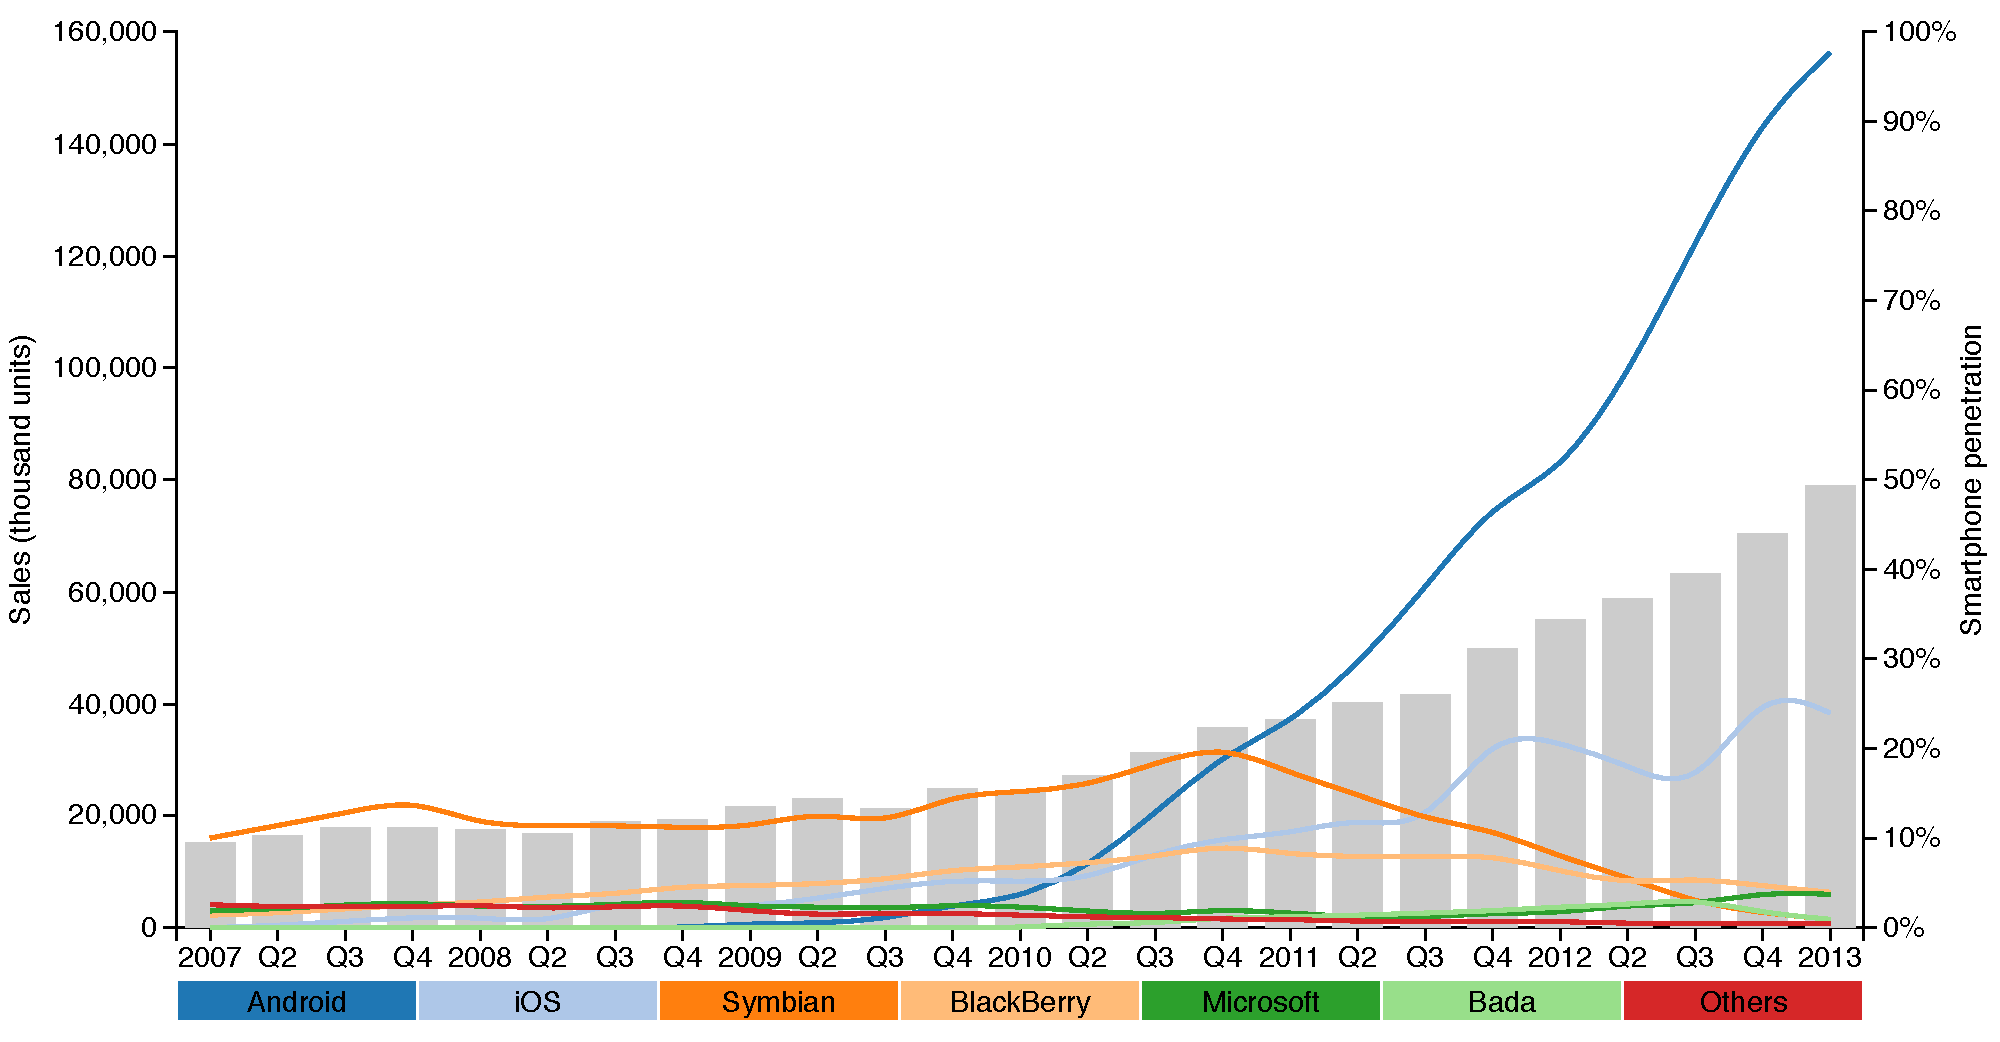
\includegraphics[width=\textwidth]{figs/smartphone_sales.pdf}
        	\caption{
        	    	Growth of worldwide smartphone sales and smartphone penetration. Source: Gartner \citep{Gartner:08Q2,Gartner:08Q3,Gartner:08Q4,Gartner:10Q1,Gartner:10Q2,Gartner:10Q3,Gartner:10Q4,Gartner:11Q1,Gartner:11Q2,Gartner:11Q3,Gartner:11Q4,Gartner:12Q1,Gartner:12Q2}
        	}
        	\label{fig:smartphone_sales}
    \end{center}
\end{figure}

\begin{figure}[h!]
    \begin{center}
        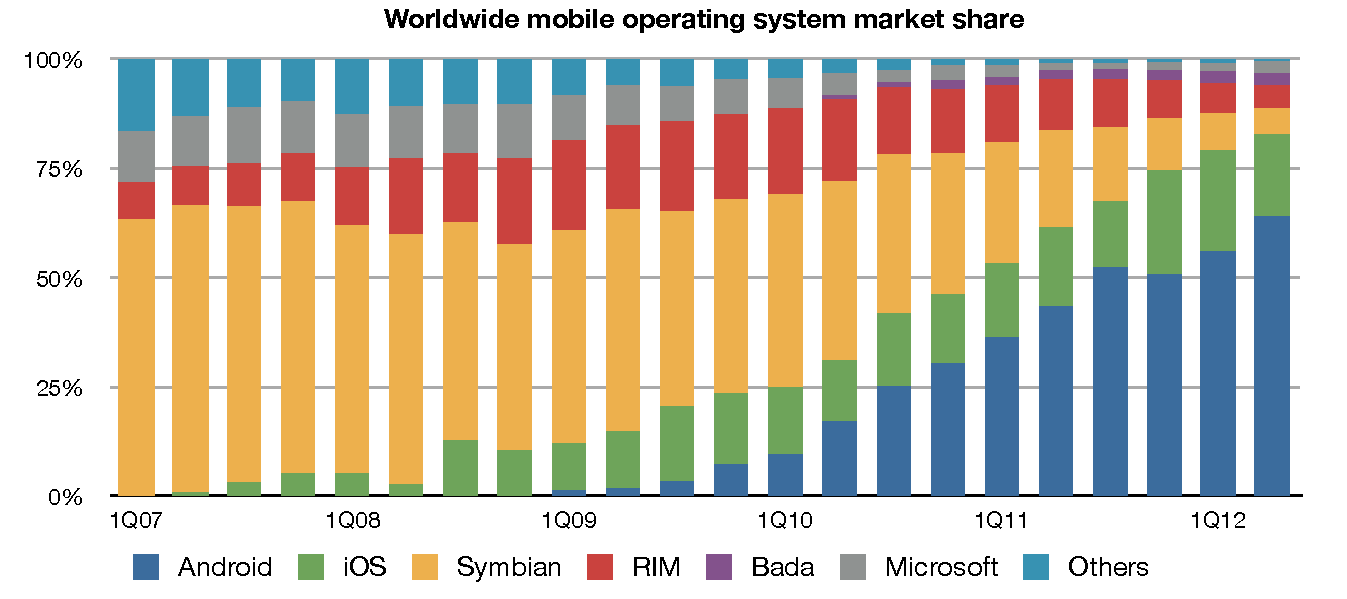
\includegraphics[width=\textwidth]{figs/smartphone_os.pdf}
        \caption{
            Growth of worldwide smartphone operating system market share. Source: Gartner \citep{Gartner:08Q2,Gartner:08Q3,Gartner:08Q4,Gartner:10Q1,Gartner:10Q2,Gartner:10Q3,Gartner:10Q4,Gartner:11Q1,Gartner:11Q2,Gartner:11Q3,Gartner:11Q4,Gartner:12Q1,Gartner:12Q2}
        	}
        \label{fig:smartphone_os}
    \end{center}
\end{figure}

But more importantly, one can conclude that there is not one major platform. Projections by the IDC show that in 2016, there will be at least three major platforms covering 90\% of the worldwide smartphone market \citep{IDC:phone}. 

A similar scenario is playing in the tablet industry. According to other studies by both Gartner \citep{Gartner:11tab,Gartner:12tab} and IDC \citep{IDC:tablet}, tablets will continue to gain popularity and sales will be mainly driven by iPads and Android tablets (see \fref{fig:tablet}).

\begin{figure}[h!]
    \begin{center}
        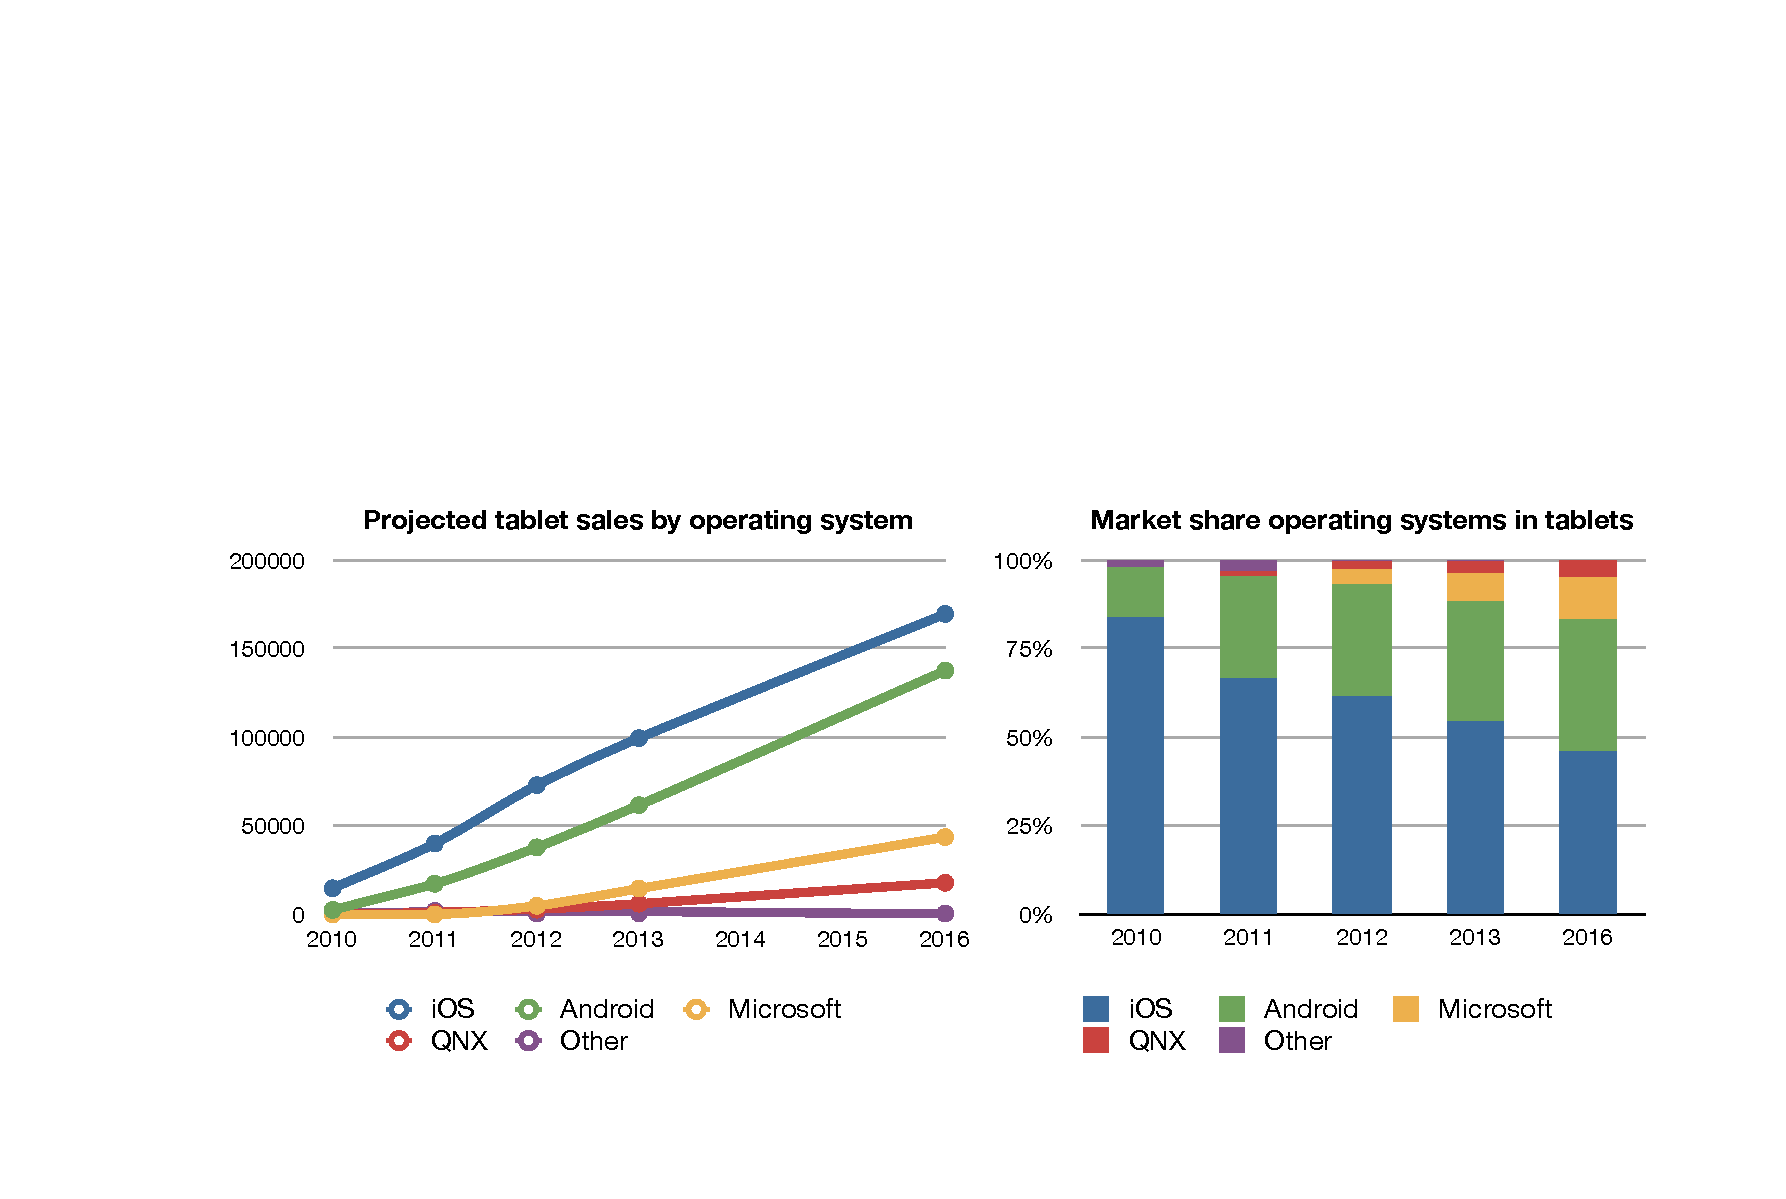
\includegraphics[width=\textwidth]{figs/tablet.pdf}
        \caption{
            Growth of worldwide smartphone sales and smartphone penetration. Source: Gartner \citep{Gartner:11tab,Gartner:12tab}
        }
        \label{fig:tablet}
    \end{center}
\end{figure}

Even though both companies do not agree on which platform will be the biggest by 2016, they both predict there will be at least three major platforms; iOS, Android and Windows. 

% TODO: summary?

\section{The problem of fragmentation}

The competition among mobile device manufacturers has led to fragmentation on many levels. For consumers, fragmentation is usually a good thing. The more different devices there are, the easier it is for a consumer to pick one that fits his needs. For developers on the other hand, fragmentation is usually considered bad. Developers have to develop and test their applications on multiple devices to be able to guarantee the desired experience. This is expensive and time consuming.

From \fref{fig:smartphone_os} and \fref{fig:tablet} it is already clear that the market is divided by operating system or platform but even within these platforms, fragmentation is multi-dimensional \citep{Kindel}.

In general, there are fewer fragmentation problems with Apple's iOS because it is a closed platform. Android, however, is an open source platform and vendors are allowed to tailor it for their devices. As a result, there are hundreds of Android based devices but also hundreds of Android flavours.

Maintenance of such Android flavours is expensive and for this reason, manufacturers do not often provide updates for their devices. This has led to noticeable runtime fragmentation among Android based devices (see \fref{fig:runtime_fragmentation}). Compared to iOS, this is a serious issue.

\begin{figure}[h!]
    \begin{center}
        \label{fig:runtime_fragmentation}
        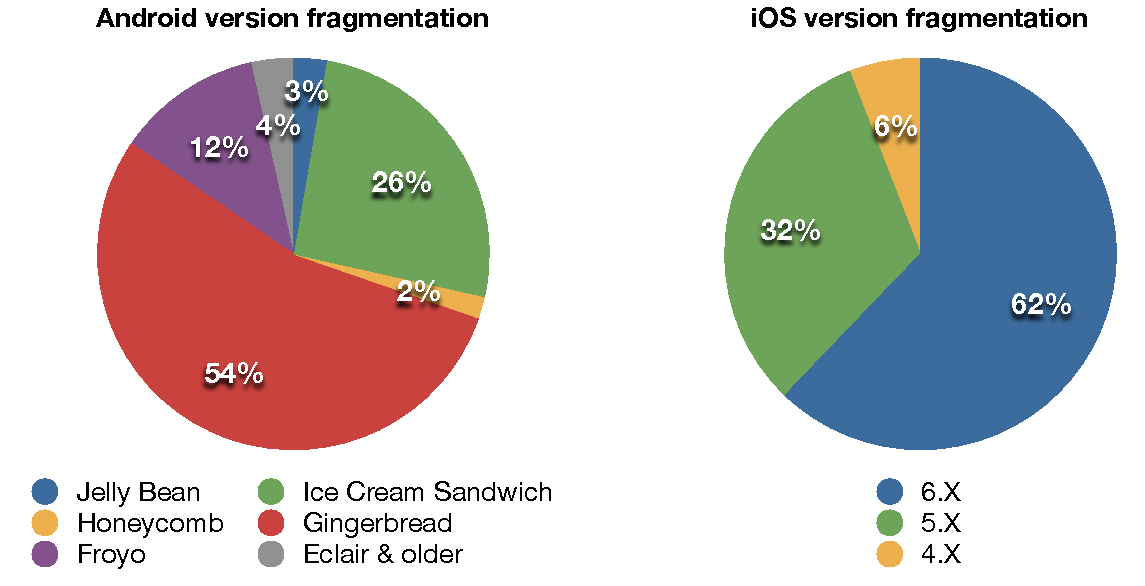
\includegraphics[width=0.8\textwidth]{figs/os_distribution.pdf}
        \caption{
            Runtime fragmentation for Android (data collected by Google during a 14-day period ending on November 1, 2012) \citep{android_distribution} and iOS (based on the statistics of developer David Smith) \citep{ios_distribution}.
        }
    \end{center}
\end{figure}

Fragmentation on the device axis is unavoidable but, again, fragmentation among Android based devices is worse than among iDevices. The most relevant items on this axis are the different hardware specifications and screen resolution.



